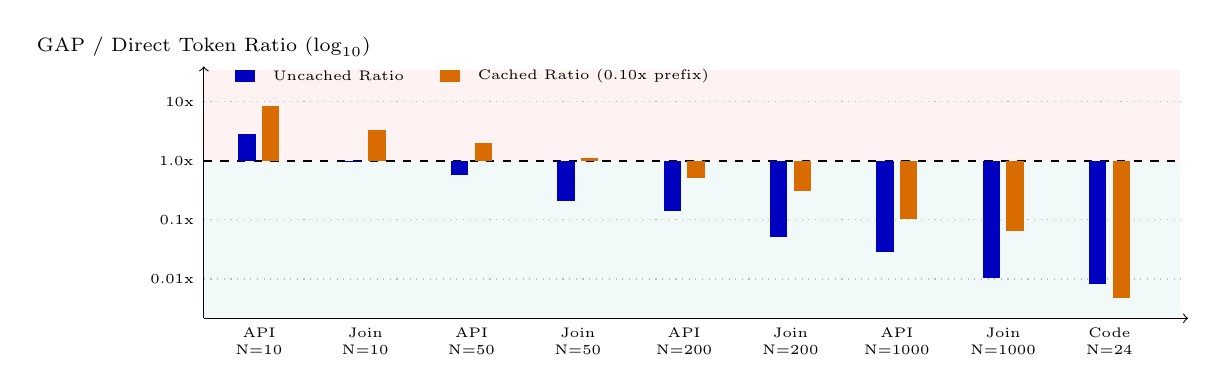
\begin{tikzpicture}[x=1cm, y=1cm]
  \fill[red!5] (0,2.000) rectangle (12.4,3.15);
  \fill[teal!5] (0,0) rectangle (12.4,2.000);
  \draw[->] (0,0) -- (12.5,0);
  \draw[->] (0,0) -- (0,3.2) node[above, font=\scriptsize] {GAP / Direct Token Ratio ($\log_{10}$)};
  \draw[dashed, thick] (0,2.000) node[left, font=\tiny] {1.0x} -- (12.4,2.000);
  \draw[dotted, gray!50] (0,0.500) node[left, font=\tiny, text=black] {0.01x} -- (12.4,0.500);
  \draw[dotted, gray!50] (0,1.250) node[left, font=\tiny, text=black] {0.1x} -- (12.4,1.250);
  \draw[dotted, gray!50] (0,2.750) node[left, font=\tiny, text=black] {10x} -- (12.4,2.750);
  \fill[blue!75!black] (0.44,2.000) rectangle (0.66,2.341);
  \fill[orange!85!black] (0.74,2.000) rectangle (0.96,2.700);
  \node[below, font=\tiny, align=center] at (0.70,0) {API\\N=10};
  \fill[blue!75!black] (1.79,1.986) rectangle (2.01,2.000);
  \fill[orange!85!black] (2.09,2.000) rectangle (2.31,2.394);
  \node[below, font=\tiny, align=center] at (2.05,0) {Join\\N=10};
  \fill[blue!75!black] (3.14,1.819) rectangle (3.36,2.000);
  \fill[orange!85!black] (3.44,2.000) rectangle (3.66,2.223);
  \node[below, font=\tiny, align=center] at (3.40,0) {API\\N=50};
  \fill[blue!75!black] (4.49,1.485) rectangle (4.71,2.000);
  \fill[orange!85!black] (4.79,2.000) rectangle (5.01,2.031);
  \node[below, font=\tiny, align=center] at (4.75,0) {Join\\N=50};
  \fill[blue!75!black] (5.84,1.369) rectangle (6.06,2.000);
  \fill[orange!85!black] (6.14,1.782) rectangle (6.36,2.000);
  \node[below, font=\tiny, align=center] at (6.10,0) {API\\N=200};
  \fill[blue!75!black] (7.19,1.039) rectangle (7.41,2.000);
  \fill[orange!85!black] (7.49,1.621) rectangle (7.71,2.000);
  \node[below, font=\tiny, align=center] at (7.45,0) {Join\\N=200};
  \fill[blue!75!black] (8.54,0.845) rectangle (8.76,2.000);
  \fill[orange!85!black] (8.84,1.261) rectangle (9.06,2.000);
  \node[below, font=\tiny, align=center] at (8.80,0) {API\\N=1000};
  \fill[blue!75!black] (9.89,0.516) rectangle (10.11,2.000);
  \fill[orange!85!black] (10.19,1.109) rectangle (10.41,2.000);
  \node[below, font=\tiny, align=center] at (10.15,0) {Join\\N=1000};
  \fill[blue!75!black] (11.24,0.442) rectangle (11.46,2.000);
  \fill[orange!85!black] (11.54,0.260) rectangle (11.76,2.000);
  \node[below, font=\tiny, align=center] at (11.50,0) {Code\\N=24};
  \fill[blue!75!black] (0.4,3.0) rectangle (0.65,3.15) node[right, xshift=3pt, yshift=-2pt, font=\tiny, text=black] {Uncached Ratio};
  \fill[orange!85!black] (3.0,3.0) rectangle (3.25,3.15) node[right, xshift=3pt, yshift=-2pt, font=\tiny, text=black] {Cached Ratio (0.10x prefix)};
\end{tikzpicture}
